
\chapter{Marco Teórico}

\label{chap2:marco-teorico}

\section{Introducción}

\label{sec21:introduccion}En este capitulo, se resumen las cuatro
áreas principales de estudio relacionados a los sistemas \abbr{HAR}
con miras a definir el problema del reconocimiento de actividades
humanas desde un punto de vista teórico. La descripción de estas áreas
detallan las aplicaciones que motivan los sistemas \abbr{HAR} y también
los mecanismos que llevan a una implementación factible. 

La primera sección, se introducen las aplicaciones de contexto que
son el principal marco de trabajo del estudio de sistemas \abbr{HAR}.
En síntesis, nuestro enfoque es detectar las actividades físicas para
dar información de contexto en las actividades diarias de un individuo
durante su locomoción. Las siguientes secciones dan todos los elementos
requeridos para implementar los sistemas \abbr{HAR}. Desde el punto
de vista de implementación se discuten los sensores y los teléfonos
móviles inteligentes. La última sección define el marco teórico del
reconocimiento de actividades humanas en base al estado del arte.

\section{Aplicaciones de contexto}

\label{sec22:contexto}En la actualidad construir aplicaciones interactivas
requieren tener en cuenta el aspecto del contexto del usuario principalmente
por la importancia de este asunto debido a que este cambia con mucha
frecuencia, como ocurren en la computación móvil y ubicua. El contexto
de un usuario es un medio adicional para la interacción entre computadora
y humano, además de otros los métodos convencionales de entrada de
datos. Este nuevo medio abre nuevas posibilidades de comunicación
y producción de nuevos servicios en computación. 

Pero, ¿qué es el contexto?, citando otras fuentes podemos definir
el contexto como: \textquotedbl{}\emph{... cualquier información que
pueda ser utilizada para caracterizar la situación de una entidad.
Un entidad es una persona, lugar, o objeto que es considerado relevante
en la interacción entre el usuario y la aplicación, incluyendo al
usuario y la aplicación}\textquotedbl{} \cite{Dey2000}. De manera
específica, el contexto de un usuario es el estado de su información
física, emocional o social, sin dejar de lado cualquier otra situación
en que el usuario esté involucrado y sea relevante para la aplicación.

Debido a la libertad de movilidad presentes en la computación móvil
y ubicua, es primordial construir aplicaciones que conozcan el contexto
de sus usuarios (\emph{context-aware}, o aplicaciones de contexto).
Debido a que el entorno de ejecución cambia con cierto dinamismo,
el rango de situaciones posibles del usuario se amplia y por lo tanto
se requiere que los servicios proveídos por una aplicación se adapten
para mejorar la interacción entre el usuario y el computador. 

Los tipos de contexto prácticos más importantes en las aplicaciones
de contexto con computación móvil son la ubicación, la identidad,
la actividad y el tiempo. Esta caracterización permite a los diseñadores
de aplicaciones escoger el contexto más relevante para su uso.

\section{Sensores}

\label{sec23:sensores} En la problemática del reconocimiento de la
actividad que está realizando una persona uno de los puntos importantes
a considerar es la elección de los sensores a utilizar. Los sensores
pueden medir signos vitales (ritmo cardíaco, temperatura del cuerpo,
presión arterial), el ambiente (intensidad de luz, temperatura, niveles
de sonido), movimiento (aceleración, velocidad), y posición (localización
global o en interiores). Sobre la localización de los sensores respecto
a la persona, algunos autores \cite{ReyesOrtiz2015} diferencian entre
ambientales, cuando los sensores esta ubicados de manera estática
en el ambiente que rodea a la persona, y \emph{wearables} cuando lo
sensores se usan o están conectados al cuerpo de la persona.

\subsection{Sensores Ambientales}

Los sensores ambientales, también denominados externos o de entorno,
son un conjunto de dispositivos que se encuentran en el medio ambiente
que miden propiedades físicas del entorno donde las personas se encuentras
e interactúan. Existe una amplia variedad de sensores ambientales,
como micrófonos, cámaras de vídeo, sensores de presencia, termómetros
y sensores de profundidad (Kinect). Para este tipo de reconocimiento
tenemos por ejemplo a \cite{Poppe2007} que realiza un análisis de
movimientos humanos utilizando cámaras de vídeo.

\subsection{Sensores Wearables}

Los sensores \emph{wearables} son usados para obtener señales directamente
en una persona, estos pueden estar unidos a varias partes del cuerpo,
como ser la cintura, muñeca, pecho, pierna, y cabeza \cite{Bao2004}
pero también pueden formar parte de la ropa o embebido en otro accesorio
de uso común, como relojes, anteojos y teléfonos móviles. Como característica
tienen una batería que proporciona la energía para poder operar, y
algunos cuentan con conexiones inalámbricas (con WIFI/Bluetooh) para
la transmisión de los datos obtenidos.

Las señales de movimiento y fisiológicas son obtenidas por los sensores,
como ser temperatura de la piel, frecuencia cardíaca, conductividad,
y posicionamiento global (\abbr{GPS}), posicionamiento en interiores
y movimientos del cuerpo. Todos estas mediciones son útiles para tener
una constante información del estado de una persona en cualquier momento.

Los sensores anexos directamente a un individuo pueden caracterizarse
según los siguientes atributos \cite{LaraLabrador2013}:
\begin{description}
\item [{Ubicación}] miden datos obtenidos con las redes celulares 3G y
los satélites de navegación \abbr{GPS}. Provee información de contexto
bastante relevante acerca de la posición del individuo, además de
ciertas medidas de movimiento pero con un consumo moderado de energía.
\item [{Movimiento}] miden datos inerciales como la aceleración y la orientación
respecto a un marco de referencia relativo al dispositivo que contiene
los sensores. El acelerómetro, giroscopio y la brújula son los sensores
más comunes y utilizados para reconocimiento de actividades con un
bajo consumo de energía y buena precisión de reconocimiento \cite{Bao2004,LaraLabrador2012}.
\item [{Fisiología}] miden signos vitales del individuo como el ritmo cardíaco
(\abbr{HRM}, \emph{Hearth Rate Monitor}), la temperatura del cuerpo,
el ritmo de respiración, entre otros.
\item [{Ambiental}] miden datos externos que rodean al individuo como el
nivel de ruido, la humedad y/o la temperatura. Los sensores de luz,
cámara, micrófonos y termómetros miden estos datos. 
\end{description}

\section{Teléfonos móviles modernos}

\label{sec24:dispositivos-moviles} Los dispositivos móviles, tales
como teléfonos móviles, reproductores de música o relojes inteligentes,
han comenzado ya hace un par de años en incorporar diversos sensores.
Debido a su tamaño reducido de estos dispositivos inteligentes, su
enorme capacidad de procesamiento, la posibilidad de recibir y enviar
datos; y su omnipresencia en nuestra sociedad de hoy, lo hacen dispositivos
de preferencia para utilizarlo en la vida diaria de un usuario.

En este trabajo, investigamos posibilidades y viabilidades de tener
un servicio para obtener el contexto de la actividad física diaria
de los usuarios con teléfonos móviles.

%% TODO: Definir mejor los teléfonos móviles, no tanto los sensores

\section{Aprendizaje Automático}

\label{sec25:aprendizaje-automatico}Una de las técnicas de reconocimiento
de actividades humanas consiste en encontrar un modelo para descubrir
información a partir de los datos, es decir utilizar algoritmos de
aprendizaje automático para construir modelos que puedan inferir actividades
a partir de una gran cantidad de datos medidos con anterioridad junto
con el comportamiento deseado del usuario\cite{Chen2012}. Esta técnica
involucra la creación de modelos de clasificación probabilistas o
estadísticos, seguidos por los procesos de entrenamiento y aprendizaje.

El aprendizaje automático implica la utilización de datos como conjunto
inicial de entrenamiento para entrenar un algoritmo, uno de muchos
existentes, como redes de Bayes, máquinas de soporte-vector \abbr{SVM},
Árboles de decisión \abbr{DT}, Modelos de Markov ocultos\abbr{HMM},
y otros \cite{Rajaraman2011} (véase siguiente sección). Las ventajas
de utilizar este enfoque de reconocimiento es su capacidad de manejar
información temporal y con cierto grado de incertidumbre, pero su
desventaja es que requiere una cantidad grande de datos de entrenamiento,
por lo que puede sufrir de problemas de inicio lento y escasez de
datos.

\section{Reconocimiento de Actividades Humanas}

\label{sec25:metodologia-har} Al igual que en otras aplicaciones
de aprendizaje automático, la actividad el reconocimiento requiere
dos etapas, es decir, entrenamiento y las pruebas o evaluación.

\begin{figure}[!htbp]
\centering 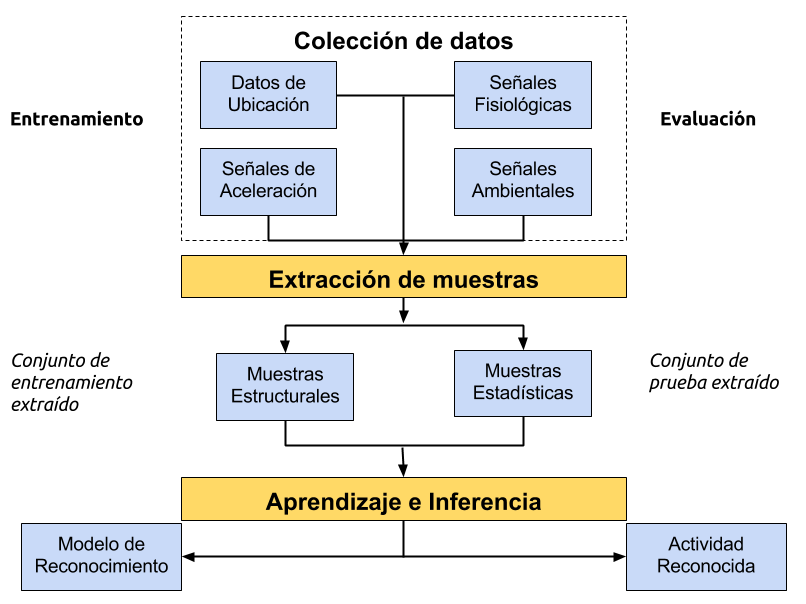
\includegraphics[width=0.7\linewidth]{capitulo-2/graphics/harsystem}
\caption[Flujo HAR]{Flujo general del Reconocimiento de Actividades Humanas}
\label{fig:harsystem} 
\end{figure}

En la \figref{fig:harsystem} se visualiza las fases comunes de las
dos etapas \cite{LaraLabrador2013}. La etapa de entrenamiento requiere
inicialmente un conjunto de datos recolectados en una serie de tiempo
con los atributos medidos a partir de individuos que realizan cada
actividad. Las series se dividen en ventanas de tiempo para aplicar
la extracción de muestras filtrando así la información relevante en
las señales en bruto. Más tarde, los métodos de aprendizaje se utilizan
para generar un modelo de reconocimiento de actividades del conjunto
de datos colectado a través de las características calculadas. Del
mismo modo, para la etapa de prueba o evaluación, se recogen datos
durante una ventana de tiempo, que se utiliza para extraer las mismas
características utilizadas en el modelo, estas se evalúan en el modelo
de aprendizaje previamente entrenado, generando una etiqueta de la
actividad predicha.

En las siguientes secciones detallamos el objetivo de la clasificación,
las responsabilidades de cada etapa y la definición formal del problema.

\subsection{Actividades Humanas}

\label{sec22:actividades-humanas} El diseño de un sistema \abbr{HAR}
depende totalmente de las actividades definidas que van a ser reconocida.
Por lo tanto, el cambio del conjunto de actividades que el sistema
reconoce convierte al problema en uno completamente diferente al anterior.

Teniendo en cuenta esto, las distintas publicaciones, tenemos estos
siete distintos grupos de actividades en la siguiente tabla.

\begin{table}[htbp]
\centering{}%
\begin{tabular}{|l|p{9cm}|}
\hline 
\textbf{Grupo}  & \textbf{Actividades} \tabularnewline
\hline 
\hline 
Ambulatoria  & Caminar, correr, sentarse, pararse, quedarse quieto, acostarse, subir
escaleras, descender escaleras, usar escaleras mecánicas, usar elevador.\tabularnewline
\hline 
Transporte  & Andar en bus, bicicleta y conducir \tabularnewline
\hline 
En el teléfono  & Enviar mensajes de texto y hacer llamadas \tabularnewline
\hline 
Actividades diarias  & Comer, beber, trabajar en la PC, mirar TV, leer, cepillarse los dientes,
aspirar el piso, y otros. \tabularnewline
\hline 
Ejercitarse  & Alzar pesas, bicicleta estática, remo y otros. \tabularnewline
\hline 
Militares  & Arrastrarse, en cuclillas, abrir la puerta \tabularnewline
\hline 
Parte superior del cuerpo  & Masticar, hablar, mover la cabeza, tragar líquidos, mirar. \tabularnewline
\hline 
\end{tabular}\caption{Grupos de Actividades.}
\label{tabla:sencilla} 
\end{table}


\subsection{Colección de Datos}

La definición del método de colección de datos es un punto importante
en un \abbr{HAR}. Según como se realiza la observación del individuo
existen: ambientes realistas, que son los ideales pero no siempre
es posible realizar este tipo de colectas. También existen los ambientes
cuasi realistas que se realizan en laboratorios simulando las condiciones
reales de las actividades. Por otro lado tenemos los ambientes totalmente
controlados en laboratorio.

Una falla en el diseño de un sistema \abbr{HAR} se puede dar por
no considerar las condiciones reales de las actividades, tales como
actividades no tenidas en cuenta, calibración de sensores, ruido,
etc.

Otra de las consideraciones a tener en cuenta en este punto es la
cantidad de individuos para realizar la colección, es recomendable
el mayor cantidad de individuos en distintos tipos de edades y condiciones
físicas.

\subsection{Extracción de Muestras}

Para cualquier problema de aprendizaje automático, la selección de
características se refiere al proceso de selección de un conjunto
significativo de características que aporten relevancia a la capacidad
de discriminación en un algoritmo de aprendizaje. Por otro lado, la
extracción de características, tiene como objetivo disminuir la cantidad
de características a utilizar mediante distintas transformaciones
entre ellas para obtener nuevas características reducidas sin perder
información relevante del conjunto de datos originales. La selección
y extracción de características también permite reducir los tiempos
de procesamiento en la fase de entrenamiento y aumenta el rendimiento
en la fase de evaluación

Dependiendo de la aplicación, las características requeridas para
la extracción de la información relevante pueden variar. En el caso
particular de \abbr{HAR}, una representación reducida de los datos
del sensor se puede utilizar como la entrada del algoritmo de reconocimiento.
Esto se logra mediante medición de la señal del sensor en varios dominios,
pudiendo ser en tiempo y frecuencia.

\subsection{Aprendizaje e Inferencia}

Varios enfoques de aprendizaje automático se han desarrollado a lo
largo de los años para resolver el problema de \abbr{HAR}. En su
mayoría a través de algoritmos de aprendizaje supervisado aunque también
se han propuesto métodos semi-supervisados y no supervisados.

Modelos de Bayes y basados en frecuencia han sido bien cubiertos en
toda la literatura \abbr{HAR}. Implican modelos basados en reglas
como Arboles de decisión \abbr{DT} y Selvas Aleatorias \abbr{RF},
algunos con un enfoques geométricos como vecinos cercanos \abbr{k-NN},
redes neuronales \abbr{ANN} y máquinas de soporte-vector \abbr{SVM},
y los métodos de clasificación probabilistas, por ejemplo clasificadores
de Bayes \abbr{NB}, y modelos ocultos de Markov \abbr{HMM}.

Otros aspectos relevantes para la selección del algoritmo de modelo
de aprendizaje incluyen: el consumo de energía, los requisitos de
memoria, interpretabilidad y complejidad de computo, etc. Estos aspectos
se agudizan si se utilizan dispositivos inteligentes .Como cuestión
de ejemplo, árboles de decisión podrían ser preferidos cuando se requiere
simplicidad en su implementación y \abbr{SVM} para aplicaciones de
alto rendimiento\cite{ReyesOrtiz2015}.

En el capitulo \ref{chap:Aprendizaje-Automatico} se detalla todo
lo referente a métodos de aprendizaje y los utilizados en este trabajo.

\subsection{Definición del Problema}

El marco teórico del estudio de los \abbr{HAR} no podría estar completo
sin una definición formal del problema. Considerando el objetivo y
los elementos del proceso de reconocimiento podemos definir el problema
según \cite{LaraLabrador2013}:

\newtheorem{defi}{Definición 1}

\begin{defi}(Problema HAR) Dado un conjunto $S=\{S_{0},...,S_{k-1}\}$
de $k$ series de tiempo, cada una con una medida particular de cada
atributo, y definidas en el intervalo de tiempo $I=\left[t_{\alpha},t_{\omega}\right]$,
el objetivo es encontrar una partición temporal (sub-intervalo de
tiempo) $\left\langle I_{0},...,I_{r-1}\right\rangle $ en $I$, basado
en los datos de $S$ y el conjunto de etiquetas que representan la
actividad realizada durante cada intervalo $I_{j}$ (Ej. quieto, caminando,
corriendo, etc.). 

Esto implica que cada intervalo $I_{j}$ son consecutivos, no vacíos,
no superpuestos y que ${\displaystyle \bigcup_{r-1}^{j=0}{I_{j}=I}}$
\end{defi}

Se asumen que las actividades consideradas no son realizadas simultáneamente,
como correr y caminar al mismo tiempo. Además, se debe notar que el
problema \abbr{HAR} no es factible a ser resuelto con una solución
determinista. El numero de combinaciones de valores de atributos y
actividades puede ser muy grande, inclusive infinito; y encontrar
los puntos de transición es complicado teniendo en cuenta que se desconoce
la duración cada actividad. 

Las practicas de aprendizaje automático son utilizadas para reconocer
actividades por medio de la clasificación. La utilización de las prácticas
de aprendizaje automático para resolver el problema requiere la introducción
de una definición relajada del problema \abbr{HAR} que sigue: 

\newtheorem{defi}{Definición 2}

\begin{defi}(Problema HAR relajado) Dado (1) un conjunto $W=\{W_{0},...,W_{m-1}\}$
de $m$ ventanas de tiempo del mismo tamaño, donde cada una esta total
o parcialmente etiquetada, y que cada $W_{i}$ contiene un conjunto
de series de tiempo $S_{i}=\{S_{i,0},...,S_{i,k-1}\}$ para cada $k$
de atributos medidos, y (2) un conjunto $A\text{=}\{a_{0},...,a_{n-1}\}$
de etiquetas de actividades, el objetivo es encontrar una función
$f\colon S_{i}\rightarrow A$ que pueda ser evaluada para todos los
valores posibles de $S_{i}$, tal que $f(S_{i})$ es lo más próximo
a la actividad realizada durante $W_{i}$ \end{defi}

Utilizar esta definición relajada introduce un error en el modelo
durante las ventanas de transición entre actividades, debido a que
en una ventana de tiempo una persona puede estar realizando más de
una actividad. Sin embargo, el número de ventanas en transición es
menor al número total de ventanas por lo que el error introducido
por la relajación no es significativo para la mayoría de las aplicaciones.

\section{Conclusión}

\label{sec27:conclusion}Este capitulo abarcó los tópicos primordiales
del estudio del reconocimiento de las actividades humanas. Los conceptos
descritos sirven de base de conocimiento para entender el problema
de \abbr{HAR} y además permiten tener una vista general de los componentes
principales para resolver el problema. Primeramente se cubre la motivación
en base a las aplicaciones, luego los medios disponibles para construir
estos sistemas: sensores, teléfonos móviles y aprendizaje automático,
y finalmente la definición metodológica y teórica del problema. 
